\documentclass[a4paper]{article} 
\addtolength{\hoffset}{-2.25cm}
\addtolength{\textwidth}{4.5cm}
\addtolength{\voffset}{-3.25cm}
\addtolength{\textheight}{5cm}
\setlength{\parskip}{0pt}
\setlength{\parindent}{0in}

%----------------------------------------------------------------------------------------
%	PACKAGES AND OTHER DOCUMENT CONFIGURATIONS
%----------------------------------------------------------------------------------------

\usepackage{blindtext} % Package to generate dummy text
\usepackage{charter} % Use the Charter font
\usepackage[utf8]{inputenc} % Use UTF-8 encoding
\usepackage{microtype} % Slightly tweak font spacing for aesthetics
\usepackage[english, ngerman]{babel} % Language hyphenation and typographical rules
\usepackage{amsthm, amsmath, amssymb} % Mathematical typesetting
\usepackage{float} % Improved interface for floating objects
\usepackage[final, colorlinks = true, 
            linkcolor = black, 
            citecolor = black]{hyperref} % For hyperlinks in the PDF
\usepackage{graphicx, multicol} % Enhanced support for graphics
\usepackage{xcolor} % Driver-independent color extensions
\usepackage{marvosym, wasysym} % More symbols
\usepackage{rotating} % Rotation tools
\usepackage{censor} % Facilities for controlling restricted text
\usepackage{listings, style/lstlisting} % Environment for non-formatted code, !uses style file!
\usepackage{pseudocode} % Environment for specifying algorithms in a natural way
\usepackage{style/avm} % Environment for f-structures, !uses style file!
\usepackage{booktabs} % Enhances quality of tables
\usepackage{tikz-qtree} % Easy tree drawing tool
\tikzset{every tree node/.style={align=center,anchor=north},
         level distance=2cm} % Configuration for q-trees
\usepackage{style/btree} % Configuration for b-trees and b+-trees, !uses style file!
\usepackage[backend=biber,style=numeric,
            sorting=nyt]{biblatex} % Complete reimplementation of bibliographic facilities
\addbibresource{ecl.bib}
\usepackage{csquotes} % Context sensitive quotation facilities
\usepackage[yyyymmdd]{datetime} % Uses YEAR-MONTH-DAY format for dates
\renewcommand{\dateseparator}{-} % Sets dateseparator to '-'
\usepackage{fancyhdr} % Headers and footers
\pagestyle{fancy} % All pages have headers and footers
\fancyhead{}\renewcommand{\headrulewidth}{0pt} % Blank out the default header
\fancyfoot[L]{} % Custom footer text
\fancyfoot[C]{} % Custom footer text
\fancyfoot[R]{\thepage} % Custom footer text
\newcommand{\note}[1]{\marginpar{\scriptsize \textcolor{red}{#1}}} % Enables comments in red on margin

%----------------------------------------------------------------------------------------

\usepackage{graphicx}
\begin{document}
\graphicspath{{home/Neil/Computing and business/Year 1/Semester 1/Java-CIS1100/Documentation/Images}}

%-------------------------------
%	TITLE SECTION
%-------------------------------

\fancyhead[C]{}
\hrule \medskip % Upper rule
\begin{minipage}{0.295\textwidth} 
\raggedright
\footnotesize
NEIL BUGEJA\hfill\\   
51000L\hfill\\
\end{minipage}
\begin{minipage}{0.4\textwidth} 
\centering 
\large 
JAVA ASSIGNMENT\\ 
\normalsize 
Machine Learning 1, 17/18\\ 
\end{minipage}
\begin{minipage}{0.295\textwidth} 
\raggedleft
\today\hfill\\
\end{minipage}
\medskip\hrule 
\bigskip

%-------------------------------
%	CONTENTS
%-------------------------------
\section{AnyClass class}
\blindtext
\subsection{First Subtask}

\bigskip

\section{Heterogeneous Circular Queue - CQueue.java}

\subsection{Construction of CQueue}
In this section a circular queue of size 20 nodes must be created. An integer called 'CIRCULAR\_QUEUE\_SIZE' is created and given the value 20. This is done so that the queue's size is stored in one location and should it need to be changed this can easily be done. \\
\\Firstly, in the Node class, two methods were created called 'getNext' and 'setNext'. These getters and setters are used below to enable the program to both get and set the pointer of the node it is given.\\
\\Secondly, a for loop is created that repeats for 'CIRCULAR\_QUEUE\_SIZE' times. In every iteration of this loop a new node is created with value null. To create this new node a method addNode is created.\\
addNode will first check whether the root is null or not. If the root is indead null, this means that the node to be implemented is the first and therefore must be classified as being the root. However, if this is not the case, the root's next will change to point towards the current node, and the current node's change will change to point towards the root. The loop will traverse the queue until it reaches the last node, guaranteeing that the queue will be circular.\\
\\The below diagram may help better illustrate what was explained above:
\bigskip

%Image:
\begin{figure}[htp]
\centering
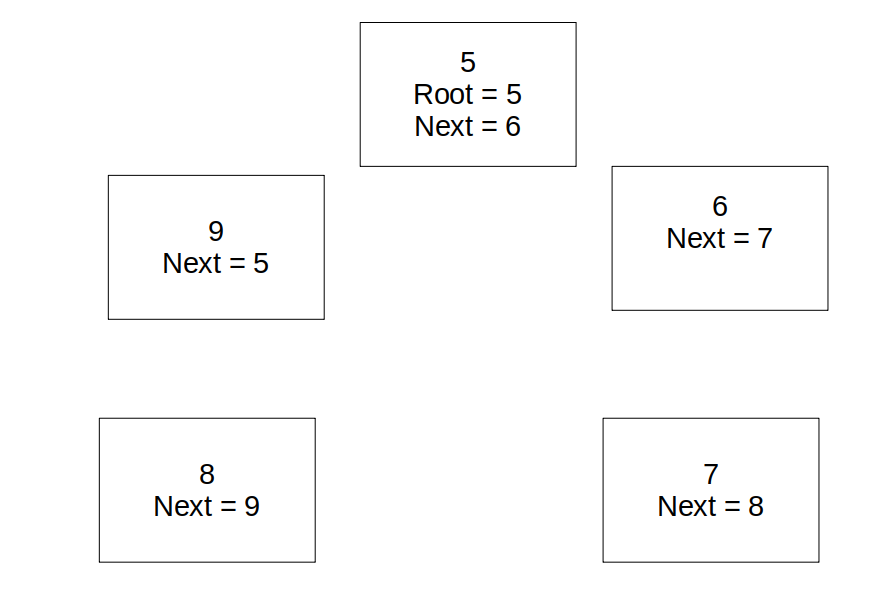
\includegraphics[scale=0.30]{Images/Insert.png}
\end{figure}

By the means of the addNode method, a circular queue is successfully created of size 'CIRCULAR\_QUEUE\_SIZE'.

\subsection{Method boolean put(AnyClass newObj)}
This method makes use of the same principles and ideas used to create the queue itself. Firstly, in the node class two methods are created which will be used to get data from a node and set data to a node.
\\Secondly, in the CQueue class, the method '\emph{put}' is created. Like the method '\emph{addNode}', it will first check if the root of the queue is null. If this is the case the root is simply filled with data by using the setter. However, if the root is not null the program will traverse the queue as it has done in the previous method to create the nodes, but this time while it is visiting a node it will set data into it.\\
\\If neither of these cases are met the method will return false, indicating that the queue is full.

\subsection{AnyClass serve()}
test. jg
test 2 again

\subsection{void listAll()}
To list all the data in the circular queue, this method will traverse by the same method that it has been doing beforehand. The only difference is that every time a node that is filled with data is encountered, it gets the data and outputs it for the user to see. By the end of the method all the data in the queue will be displayed.\\

\subsection{AnyClass editObject(String key)}
This method will once again begin by traversing the entire queue. If it encounters an array with data it will check to see if it matches with the key that the user wishes to edit. If this is the case, the key's data is acquired and used in the method edit found in Employee.java. This method is explained further down below
\bigskip

%------------------------------------------------

\section{Emplyee - Employee.java}

When declaring an employee, he must be given:
\\1. A number relating to the serial number
\\2. The employee's surname
\\3. The employee's salary which is declared as a double.\\
\\The class has the appropriate getters and setters in place to get and set salary and get the employee's key which is the surname. A method is also created which retrieves the employee's data which includes his id number, surname(key), and salary.\\
\\Lastly, another method is created which is used to edit the employee's salary. This method will first display's the employee's current salary by means of the getter, and later set a new salary by means of a setter.
\bigskip 

%------------------------------------------------
\section{PartTimer - PartTimer.java}
PartTimer extends employee as it is basically employee but with a few additions. A constructor for PartTimer is present as hours must also be declared in the case for a part time employee. The constructor makes use of supers as they are the same as employee.java. A method is present which retrieves the partTimer's hours and another method 'getData()' which overrides the method 'getData()' found in employee.java. This is important as without it the partTimer's hours cannot be viewed.
\bigskip

\section{Deliverables - Main.java}
The menu starts by first creating the CQueue which will be used to store both types of employees. Next the menu is displayed and depending on the user's choice the menu will call a different method. Below is a list of all options and how they function:
\subsection{Populate Queue}
The queue must be populated with both full time and part time employees. Therefore, the method will first ask the user how many new full time employees have to be inserted. In the case of full time employees the sequence number, surname and salary are required while part time employees must also enter their working hours as per the assignment specifications. The employees are inserted into the queue by the "put" method.
\subsection{First Subtask}
\subsection{First Subtask}
\subsection{Update payment of person}


\bigskip

%------------------------------------------------

\end{document}
